% answers.tex —— 2002 年·全国旧课程卷·文科 · 参考答案与详细解析片段
% 由 tools/generate_projects.py 依来源总账自 2002/2002_数学真题_全国旧课程文_试题.md + 2002/2002_数学真题_全国旧课程文_解析正文.md + 2002/2002_数学真题_全国旧课程文_答案要点.md 生成，勿手改（改源 MD 后重跑）


\begin{gktip}
固定源 PDF 为印刷页码 106–107 的两页题面，不附答案。以下解析均依据题面独立复算；第 13、17、19、22 题图形在 LaTeX 工程中以 TikZ/PGFPlots 矢量源重绘。
\end{gktip}

\gkpart{一、选择题}

\begin{answer}
\gksolhead{1}{}

\textbf{题目}：

直线 $(1+a)x+y+1=0$ 与圆 $x^2+y^2-2x=0$ 相切，则 $a$ 的值为\mbox{（　　）}

（A）$\pm1$　　（B）$\pm2$　　（C）$1$　　（D）$-1$

\Needspace{4\baselineskip}
\textbf{解析}

\Needspace{5\baselineskip}
圆 $x^2+y^2-2x=0$ 的圆心为 $(1,0)$、半径为 $1$。圆心到直线的距离为

\nopagebreak[4]
\[
\frac{|(1+a)+1|}{\sqrt{(1+a)^2+1}}.
\]

\Needspace{5\baselineskip}
相切时该距离等于 $1$，平方化简得

\nopagebreak[4]
\[
\bigl((1+a)+1\bigr)^2=(1+a)^2+1
\Longrightarrow 2(1+a)=0.
\]

所以 $u=0$，即 $a=-1$，选 D。

\gkanswer{答案：D}

\end{answer}
\begin{answer}
\gksolhead{2}{}

\textbf{题目}：

\Needspace{5\baselineskip}
复数

\nopagebreak[4]
\[
\left(\frac12+\frac{\sqrt3}{2}i\right)^3
\]

的值是\mbox{（　　）}

（A）$-i$　　（B）$i$　　（C）$-1$　　（D）$1$

\Needspace{4\baselineskip}
\textbf{解析}

\Needspace{5\baselineskip}
由棣莫弗定理，

\nopagebreak[4]
\[
\left(\frac12+\frac{\sqrt3}{2}i\right)^3
=\left(\cos\frac\pi3+i\sin\frac\pi3\right)^3
=\cos\pi+i\sin\pi=-1.
\]

故选 C。

\gkanswer{答案：C}

\end{answer}
\begin{answer}
\gksolhead{3}{}

\textbf{题目}：

不等式 $(1+x)(1-|x|)>0$ 的解集是\mbox{（　　）}

（A）$\{x\mid 0\leqslant x<1\}$

（B）$\{x\mid x<0\text{ \text{且} }x\neq-1\}$

（C）$\{x\mid -1<x<1\}$

（D）$\{x\mid x<1\text{ \text{且} }x\neq-1\}$

\Needspace{4\baselineskip}
\textbf{解析}

\Needspace{5\baselineskip}
当 $x\geqslant0$ 时，原不等式化为 $(1+x)(1-x)>0$，得到 $0\leqslant x<1$；当 $x<0$ 时，化为 $(1+x)^2>0$，得到 $x<0$ 且 $x\neq-1$。合并得

\nopagebreak[4]
\[
x<1,\qquad x\neq-1.
\]

故选 D。

\gkanswer{答案：D}

\end{answer}
\begin{answer}
\gksolhead{4}{}

\textbf{题目}：

函数 $y=a^x$ 在 $[0,1]$ 上的最大值与最小值之和为 $3$，则 $a=$\mbox{（　　）}

（A）$\frac12$　　（B）$2$　　（C）$4$　　（D）$\frac14$

\Needspace{4\baselineskip}
\textbf{解析}

若 $a>1$，$a^x$ 在 $[0,1]$ 上的最小值、最大值分别为 $1\text{、}a$，所以 $1+a=3$，得 $a=2$。若 $0<a<1$，最大值与最小值之和为 $1+a<2$，不可能为 $3$。故选 B。

\gkanswer{答案：B}

\end{answer}
\begin{answer}
\gksolhead{5}{}

\textbf{题目}：

在 $(0,2\pi)$ 内，使 $\sin x>\cos x$ 成立的 $x$ 的取值范围是\mbox{（　　）}

（A）$\left(\frac\pi4,\frac\pi2\right)\cup\left(\pi,\frac{5\pi}4\right)$

（B）$\left(\frac\pi4,\pi\right)$

（C）$\left(\frac\pi4,\frac{5\pi}4\right)$

（D）$\left(\frac\pi4,\pi\right)\cup\left(\frac{5\pi}4,\frac{3\pi}2\right)$

\Needspace{4\baselineskip}
\textbf{解析}

\nopagebreak[4]
\[
\sin x>\cos x
\Longleftrightarrow
\sin\left(x-\frac\pi4\right)>0.
\]

\Needspace{5\baselineskip}
在 $0<x<2\pi$ 内，解集为

\nopagebreak[4]
\[
\left(\frac\pi4,\frac{5\pi}4\right),
\]

故选 C。

\gkanswer{答案：C}

\end{answer}
\begin{answer}
\gksolhead{6}{}

\textbf{题目}：

\Needspace{5\baselineskip}
设集合

\nopagebreak[4]
\[
M=\left\{x\middle|x=\frac{k}{2}+\frac14,\ k\in\mathbb Z\right\},\qquad
N=\left\{x\middle|x=\frac{k}{4}+\frac12,\ k\in\mathbb Z\right\},
\]

则\mbox{（　　）}

（A）$M=N$　　（B）$M\subseteq N$　　（C）$M\supseteq N$　　（D）$M\cap N=\varnothing$

\Needspace{4\baselineskip}
\textbf{解析}

\nopagebreak[4]
\[
M=\left\{\frac{2k+1}{4}\middle|k\in\mathbb Z\right\},\qquad
N=\left\{\frac{j}{4}\middle|j\in\mathbb Z\right\}.
\]

因此 $M$ 中的每个元素都属于 $N$，即 $M\subseteq N$，选 B。

\gkanswer{答案：B}

\end{answer}
\begin{answer}
\gksolhead{7}{}

\textbf{题目}：

椭圆 $5x^2+ky^2=5$ 的一个焦点是 $(0,2)$，那么 $k=$\mbox{（　　）}

（A）$-1$　　（B）$1$　　（C）$\sqrt5$　　（D）$-\sqrt5$

\Needspace{4\baselineskip}
\textbf{解析}

\Needspace{5\baselineskip}
椭圆可写为

\nopagebreak[4]
\[
x^2+\frac{k}{5}y^2=1.
\]

\Needspace{5\baselineskip}
焦点在 $y$ 轴上，故 $\dfrac5k>1$，且

\nopagebreak[4]
\[
\frac5k-1=2^2.
\]

所以 $5/k=5$，得到 $k=1$，选 B。

\gkanswer{答案：B}

\end{answer}
\begin{answer}
\gksolhead{8}{}

\textbf{题目}：

一个圆锥和一个半球有公共底面，如果圆锥的体积恰好与半球的体积相等，那么这个圆锥轴截面顶角的余弦值是\mbox{（　　）}

（A）$\frac34$　　（B）$\frac45$　　（C）$\frac35$　　（D）$-\frac35$

\Needspace{4\baselineskip}
\textbf{解析}

\Needspace{5\baselineskip}
设公共底面半径为 $r$，圆锥高为 $h$。由体积相等，

\nopagebreak[4]
\[
\frac13\pi r^2h=\frac23\pi r^3,
\qquad\text{\text{故}}\qquad h=2r.
\]

\Needspace{5\baselineskip}
轴截面是底边 $2r$、高 $2r$ 的等腰三角形。若顶角为 $\gamma$，则

\nopagebreak[4]
\[
\cos\gamma
=\frac{h^2-r^2}{h^2+r^2}
=\frac{4r^2-r^2}{4r^2+r^2}
=\frac35.
\]

故选 C。

\gkanswer{答案：C}

\end{answer}
\begin{answer}
\gksolhead{9}{}

\textbf{题目}：

已知 $0<x<y<a<1$，则有\mbox{（　　）}

（A）$\log_a(xy)<0$

（B）$0<\log_a(xy)<1$

（C）$1<\log_a(xy)<2$

（D）$\log_a(xy)>2$

\Needspace{4\baselineskip}
\textbf{解析}

\Needspace{5\baselineskip}
因为 $0<x<y<a<1$，所以 $0<xy<a^2$。以 $a$ 为底的对数函数递减，因此

\nopagebreak[4]
\[
\log_a(xy)>\log_a(a^2)=2.
\]

故选 D。

\gkanswer{答案：D}

\end{answer}
\begin{answer}
\gksolhead{10}{}

\textbf{题目}：

函数 $y=x^2+bx+c$，$x\in[0,+\infty)$ 是单调函数的充要条件是\mbox{（　　）}

（A）$b\geqslant0$　　（B）$b\leqslant0$　　（C）$b>0$　　（D）$b<0$

\Needspace{4\baselineskip}
\textbf{解析}

\nopagebreak[4]
\[
y'=2x+b.
\]

在 $[0,+\infty)$ 上要使二次函数单调，只能使其始终单调递增，这等价于 $2x+b\geqslant0$ 对所有 $x\geqslant0$ 成立，也就是 $b\geqslant0$。故选 A。

\gkanswer{答案：A}

\end{answer}
\begin{answer}
\gksolhead{11}{}

\textbf{题目}：

\Needspace{5\baselineskip}
设 $\theta\in\left(0,\dfrac\pi4\right)$，则二次曲线

\nopagebreak[4]
\[
x^2\cot\theta-y^2\tan\theta=1
\]

的离心率的取值范围为\mbox{（　　）}

（A）$\left(0,\frac12\right)$　　（B）$\left(\frac12,\frac{\sqrt2}{2}\right)$

（C）$\left(\frac{\sqrt2}{2},2\right)$　　（D）$(\sqrt2,+\infty)$

\Needspace{4\baselineskip}
\textbf{解析}

\Needspace{5\baselineskip}
原方程化为

\nopagebreak[4]
\[
\frac{x^2}{\tan\theta}-\frac{y^2}{\cot\theta}=1.
\]

\Needspace{5\baselineskip}
它是双曲线，且

\nopagebreak[4]
\[
a^2=\tan\theta,\qquad b^2=\cot\theta,
\]

\Needspace{5\baselineskip}
所以离心率

\nopagebreak[4]
\[
e=\sqrt{1+\frac{b^2}{a^2}}
=\sqrt{1+\cot^2\theta}
=\frac1{\sin\theta}.
\]

当 $0<\theta<\pi/4$ 时，$0<\sin\theta<\sqrt2/2$，故 $e>\sqrt2$，选 D。

\gkanswer{答案：D}

\end{answer}
\begin{answer}
\gksolhead{12}{}

\textbf{题目}：

从正方体的 6 个面中选取 3 个面，其中有 2 个面不相邻的选法共有\mbox{（　　）}

（A）8 种　　（B）12 种　　（C）16 种　　（D）20 种

\Needspace{4\baselineskip}
\textbf{解析}

\Needspace{5\baselineskip}
先从正方体的三组相对面中选一组，有 $3$ 种；再从其余 $4$ 个面中选第三个面。所选的三个面中恰有一对相对面，因此共有

\nopagebreak[4]
\[
3\times4=12
\]

种，选 B。

\gkanswer{答案：B}

\end{answer}
\gkpart{二、填空题}

\begin{answer}
\gksolhead{13}{}

\textbf{题目}：

据新华社 2002 年 3 月 12 日电，1985 年到 2000 年间，我国农村人均居住面积如图所示，其中，从\gkblank{}年到\gkblank{}年的五年间增长最快。
\nopagebreak[4]
\begin{center}% 2002 年全国旧课程文科第 13 题：农村人均居住面积柱状图
\begin{tikzpicture}[x=0.85cm,y=0.22cm,>=stealth]
  \draw[->] (0,0)--(5.4,0) node[right] {年份};
  \draw[->] (0,0)--(0,29) node[above] {面积/$\mathrm{m^2}$};
  \foreach \y/\label in {10/10,15/15,20/20,25/25}
    \draw (-0.12,\y)--(0.12,\y) node[left=5pt] {\label};
  \foreach \x/\label in {1/1985,2.3/1990,3.6/1995,4.9/2000}
    \draw (\x,0.15)--(\x,-0.15) node[below=4pt] {\label};
  \foreach \x/\h/\label in {
    1/14.7/14.7,
    2.3/17.8/17.8,
    3.6/21.0/21.0,
    4.9/24.8/24.8}
  {
    \draw[fill=gray!25] (\x-0.32,0) rectangle (\x+0.32,\h);
    \node[above=3pt] at (\x,\h) {\label};
  }
\end{tikzpicture}
\end{center}
\nopagebreak[4]
\begin{center}
\begin{tabular}{lrrrr}
\toprule
年份 & 1985 & 1990 & 1995 & 2000 \\
\midrule
人均居住面积（$\mathrm{m^2}$） & 14.7 & 17.8 & 21.0 & 24.8 \\
\bottomrule
\end{tabular}
\end{center}

\Needspace{4\baselineskip}
\textbf{解析}

\Needspace{5\baselineskip}
相邻两个五年段的人均居住面积增长量分别为

\nopagebreak[4]
\[
17.8-14.7=3.1,\qquad
21.0-17.8=3.2,\qquad
24.8-21.0=3.8.
\]

最大增长量出现在 1995 年到 2000 年。

\gkanswer{答案：1995—2000}

\end{answer}
\begin{answer}
\gksolhead{14}{}

\textbf{题目}：

\Needspace{5\baselineskip}
函数

\nopagebreak[4]
\[
y=\frac{2x}{1+x},\qquad x\in(-1,+\infty)
\]

图象与其反函数图象的交点为\gkblank{}。

\Needspace{4\baselineskip}
\textbf{解析}

\Needspace{5\baselineskip}
设交点同时在函数图象和反函数图象上，则它必须在直线 $y=x$ 上。代入原函数：

\nopagebreak[4]
\[
x=\frac{2x}{1+x}
\Longleftrightarrow x(x-1)=0.
\]

\Needspace{5\baselineskip}
两点均在定义域内，故交点为

\nopagebreak[4]
\[
(0,0),\qquad(1,1).
\]

\gkanswer{答案：$(0,0),(1,1)$}

\end{answer}
\begin{answer}
\gksolhead{15}{}

\textbf{题目}：

$(x^2+1)(x-2)^7$ 展开式中 $x^3$ 的系数是\gkblank{}。

\Needspace{4\baselineskip}
\textbf{解析}

\Needspace{5\baselineskip}
所求系数由两部分组成：

\nopagebreak[4]
\[
[x^3]\bigl((x^2+1)(x-2)^7\bigr)
=[x](x-2)^7+[x^3](x-2)^7.
\]

\Needspace{5\baselineskip}
其中

\nopagebreak[4]
\[
[x](x-2)^7=\binom71(-2)^6=448,
\]

\nopagebreak[4]
\[
[x^3](x-2)^7=\binom73(-2)^4=560.
\]

所以所求系数为 $448+560=1008$。

\gkanswer{答案：$1008$}

\end{answer}
\begin{answer}
\gksolhead{16}{}

\textbf{题目}：

对于顶点在原点的抛物线，给出下列条件：

① 焦点在 $y$ 轴上；

② 焦点在 $x$ 轴上；

③ 抛物线上横坐标为 $1$ 的点到焦点的距离等于 $6$；

④ 抛物线的通径的长为 $5$；

⑤ 由原点向过焦点的某条直线作垂线，垂足坐标为 $(2,1)$。

能使这抛物线方程为 $y^2=10x$ 的条件是\gkblank{}。（要求填写合适条件的序号）

\Needspace{4\baselineskip}
\textbf{解析}

抛物线 $y^2=10x$ 的焦点为 $(5/2,0)$。

\Needspace{5\baselineskip}
焦点在 $x$ 轴上，所以条件②成立；通径长为 $10$，不是 $5$，故条件④不成立。横坐标为 $1$ 的点到焦点的距离为

\nopagebreak[4]
\[
\sqrt{\left(1-\frac52\right)^2+10}=\frac72,
\]

故条件③不成立。

\Needspace{5\baselineskip}
对于条件⑤，过垂足 $(2,1)$ 且垂直于 $O(2,1)$ 的直线为

\nopagebreak[4]
\[
2x+y-5=0.
\]

焦点 $(5/2,0)$ 在此直线上，故条件⑤也成立。因此填②⑤。

\gkanswer{答案：②⑤}

\end{answer}
\gkpart{三、解答题}

\begin{answer}
\gksolhead{17}{}

\textbf{题目}：

\Needspace{5\baselineskip}
如图，某地一天从 6 时至 14 时的温度变化曲线近似满足函数

\nopagebreak[4]
\[
y=A\sin(\omega x+\varphi)+b.
\]
\nopagebreak[4]
\begin{center}% 2002 年全国旧课程文科第 17 题：温度变化曲线
\begin{tikzpicture}[x=0.62cm,y=0.13cm,>=stealth]
  \draw[->] (5.2,0)--(14.8,0) node[right] {$t/\mathrm h$};
  \draw[->] (5.2,0)--(5.2,34) node[above] {$T/{}^\circ\mathrm C$};
  \foreach \y in {10,20,30}
    \draw[dashed,gray] (5.2,\y)--(14,\y) node[right] {\y};
  \foreach \x in {6,8,10,12,14}
    \draw (\x,0.4)--(\x,-0.4) node[below=3pt] {\x};
  \draw[thick,domain=6:14,samples=80]
    plot (\x,{20+10*sin(22.5*(\x-10))});
  \node[below left] at (5.2,0) {$O$};
\end{tikzpicture}
\end{center}
\nopagebreak[4]
（1） 求这段时间的最大温差；

（2） 写出这段时间的函数解析式。

\Needspace{4\baselineskip}
\textbf{解析}

\gksubpart{(1)}

\Needspace{5\baselineskip}
由图可读出在 $6$ 时和 $14$ 时的温度分别为 $10^\circ\mathrm C$、$30^\circ\mathrm C$，中点 $10$ 时的温度为 $20^\circ\mathrm C$。因此最大温差为

\nopagebreak[4]
\[
30-10=20^\circ\mathrm C.
\]

\Needspace{5\baselineskip}
取中线为 $T=20$，振幅为 $10$。从 $t=10$ 到 $t=14$ 恰为四分之一周期，故

\nopagebreak[4]
\[
\omega(14-10)=\frac\pi2,\qquad \omega=\frac\pi8.
\]

\gksubpart{(2)}

\Needspace{5\baselineskip}
令 $t=10$ 时相位为 $0$，得到

\nopagebreak[4]
\[
T=10\sin\left(\frac\pi8(t-10)\right)+20,
\qquad 6\leqslant t\leqslant14.
\]

\gkanswer{答案（1）：$20^\circ\mathrm C$。}

\gkanswer{答案（2）：$T=10\sin\left(\dfrac\pi8(t-10)\right)+20$，$6\leqslant t\leqslant14$。}

\end{answer}
\begin{answer}
\gksolhead{18}{}

\textbf{题目}：

甲、乙物体分别从相距 70 米的两处同时相向运动。甲第 1 分钟走 2 米，以后每分钟比前 1 分钟多走 1 米，乙每分钟走 5 米。

（1） 甲、乙开始运动后几分钟相遇？

（2） 如果甲、乙到达对方起点后立即折返，甲继续每分钟比前 1 分钟多走 1 米，乙继续每分钟走 5 米，那么开始运动几分钟后第二相遇？

\Needspace{4\baselineskip}
\textbf{解析}

\Needspace{5\baselineskip}
甲第 $n$ 分钟走 $n+1$ 米，因此前 $n$ 分钟走过的路程为

\nopagebreak[4]
\[
S_n=2+3+\cdots+(n+1)=\frac{n(n+3)}2.
\]

\gksubpart{(1)}

\Needspace{5\baselineskip}
第一次相遇时两物体共走完 $70$ 米，所以

\nopagebreak[4]
\[
\frac{n(n+3)}2+5n=70.
\]

\Needspace{5\baselineskip}
化简得

\nopagebreak[4]
\[
n^2+13n-140=0,
\]

取正根得 $n=7$。所以第一次相遇在开始运动后 $7$ 分钟。

\gksubpart{(2)}

\Needspace{5\baselineskip}
乙每分钟走 $5$ 米，恰好在第 $14$ 分钟到达甲的起点并立即折返。甲前 $14$ 分钟若不折返共走

\nopagebreak[4]
\[
S_{14}=\frac{14(14+3)}2=119
\]

米；甲此前已经到达乙的起点并折返，所以第 $14$ 分钟末的位置为 $140-119=21$ 米（从甲的起点量起）。

\Needspace{5\baselineskip}
在第 $15$ 分钟内，甲的速度为 $16$ 米/分钟。设第二次相遇时间为 $t$，且 $14\leqslant t\leqslant15$，则两者位置分别为

\nopagebreak[4]
\[
140-\bigl(119+16(t-14)\bigr),\qquad 5(t-14).
\]

\Needspace{5\baselineskip}
令两式相等：

\nopagebreak[4]
\[
21-16(t-14)=5(t-14)
\Longrightarrow t-14=1.
\]

故第二次相遇发生在开始运动后 $15$ 分钟。

\gkanswer{答案（1）：7 分钟。}

\gkanswer{答案（2）：15 分钟。}

\end{answer}
\begin{answer}
\gksolhead{19}{}

\textbf{题目}：

四棱锥 $P-ABCD$ 的底面是边长为 $a$ 的正方形，$PB\perp$ 平面 $ABCD$。
\nopagebreak[4]
\begin{center}% 2002 年全国旧课程文科第 19 题：四棱锥 P-ABCD
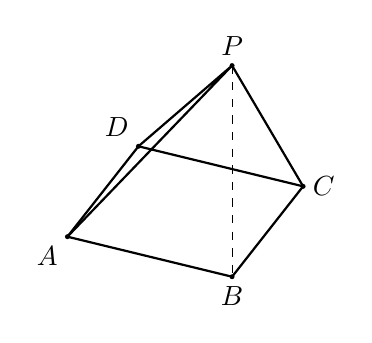
\begin{tikzpicture}[>=stealth,scale=0.82]
  \coordinate (A) at (0,0);
  \coordinate (B) at (2.55,-0.62);
  \coordinate (C) at (3.65,0.78);
  \coordinate (D) at (1.10,1.40);
  \coordinate (P) at (2.55,2.65);
  \draw[thick] (A)--(B)--(C)--(D)--cycle;
  \draw[thick] (P)--(A) (P)--(C) (P)--(D);
  \draw[dashed] (P)--(B);
  \fill (A) circle (1.1pt) node[below left] {$A$};
  \fill (B) circle (1.1pt) node[below] {$B$};
  \fill (C) circle (1.1pt) node[right] {$C$};
  \fill (D) circle (1.1pt) node[above left] {$D$};
  \fill (P) circle (1.1pt) node[above] {$P$};
\end{tikzpicture}
\end{center}
\nopagebreak[4]
（1） 若面 $PAD$ 与面 $ABCD$ 所成的二面角为 $60^\circ$，求这个四棱锥的体积；

（2） 证明无论四棱锥的高怎样变化，面 $PAD$ 与面 $PCD$ 所成的二面角恒大于 $90^\circ$。

\Needspace{4\baselineskip}
\textbf{解析}

\Needspace{5\baselineskip}
建立空间直角坐标系，令

\nopagebreak[4]
\[
A=(0,0,0),\quad B=(a,0,0),\quad C=(a,a,0),\quad D=(0,a,0),\quad P=(a,0,h),
\]

其中 $h=PB>0$。

\gksubpart{(1)}

由于 $AB\perp AD$ 且 $PB\perp$ 平面 $ABCD$，有 $PA\perp AD$。因此 $\angle PAB$ 是面 $PAD$ 与面 $ABCD$ 所成二面角的平面角。

\Needspace{5\baselineskip}
题设给出 $\angle PAB=60^\circ$，所以

\nopagebreak[4]
\[
\tan60^\circ=\frac{PB}{AB}=\frac ha,
\qquad h=a\sqrt3.
\]

\Needspace{5\baselineskip}
四棱锥体积为

\nopagebreak[4]
\[
V=\frac13\cdot a^2\cdot a\sqrt3
=\frac{\sqrt3}{3}a^3.
\]

\gksubpart{(2)}

\Needspace{5\baselineskip}
面 $PAD$ 的一个法向量可取

\nopagebreak[4]
\[
\boldsymbol n_1=(h,0,-a),
\]

\Needspace{5\baselineskip}
面 $PCD$ 的一个法向量可取

\nopagebreak[4]
\[
\boldsymbol n_2=(0,h,a).
\]

\Needspace{5\baselineskip}
两法向量的内积为

\nopagebreak[4]
\[
\boldsymbol n_1\cdot\boldsymbol n_2=-a^2<0,
\]

\Needspace{5\baselineskip}
且

\nopagebreak[4]
\[
|\boldsymbol n_1|=|\boldsymbol n_2|=\sqrt{h^2+a^2}.
\]

\Needspace{5\baselineskip}
因此两面所成的相应二面角 $\beta$ 满足

\nopagebreak[4]
\[
\cos\beta
=\frac{-a^2}{h^2+a^2}<0.
\]

从而 $\beta>90^\circ$，且结论与 $h$ 的具体取值无关。

\gkanswer{答案（1）：$\dfrac{\sqrt3}{3}a^3$。}

\gkanswer{答案（2）：见解析版。}

\end{answer}
\begin{answer}
\gksolhead{20}{}

\textbf{题目}：

\Needspace{5\baselineskip}
设函数

\nopagebreak[4]
\[
f(x)=x^2+|x-2|-1,\qquad x\in\mathbb R.
\]

（1） 判断 $f(x)$ 的奇偶性；

（2） 求函数 $f(x)$ 的最小值。

\Needspace{4\baselineskip}
\textbf{解析}

\Needspace{5\baselineskip}
分段写出函数：

\nopagebreak[4]
\[
f(x)=
\begin{cases}
x^2-x+1,&x<2,\\
x^2+x-3,&x\geqslant2.
\end{cases}
\]

\gksubpart{(1)}

取 $f(1)=1$、$f(-1)=3$，可知 $f(-1)\neq f(1)$，所以它不是偶函数；又 $f(0)=1\neq0$，所以它不是奇函数。

\gksubpart{(2)}

\Needspace{5\baselineskip}
在 $x<2$ 时，

\nopagebreak[4]
\[
x^2-x+1=\left(x-\frac12\right)^2+\frac34,
\]

\Needspace{5\baselineskip}
最小值为 $3/4$，在 $x=1/2$ 处取得。第二段在 $x\geqslant2$ 上的最小值为 $3$，故全函数最小值为

\nopagebreak[4]
\[
\frac34.
\]

\gkanswer{答案（1）：既不是奇函数，也不是偶函数。}

\gkanswer{答案（2）：$\dfrac34$。}

\end{answer}
\begin{answer}
\gksolhead{21}{}

\textbf{题目}：

已知点 $P$ 到两定点 $M(-1,0)\text{、}N(1,0)$ 距离的比为 $\sqrt2$，点 $N$ 到直线 $PM$ 的距离为 $1$，求直线 $PN$ 的方程。

\Needspace{4\baselineskip}
\textbf{解析}

\Needspace{5\baselineskip}
按题面顺序理解距离比为

\nopagebreak[4]
\[
\frac{PM}{PN}=\sqrt2.
\]

\Needspace{5\baselineskip}
设 $P=(x,y)$。直线 $PM$ 的方程为

\nopagebreak[4]
\[
yX-(x+1)Y+y=0.
\]

\Needspace{5\baselineskip}
点 $N(1,0)$ 到此直线的距离为

\nopagebreak[4]
\[
\frac{2|y|}{PM}=1,
\qquad\text{\text{故}}\qquad PM=2|y|.
\]

\Needspace{5\baselineskip}
由 $PM/PN=\sqrt2$ 得

\nopagebreak[4]
\[
PN=\sqrt2\,|y|.
\]

\Needspace{5\baselineskip}
于是

\nopagebreak[4]
\[
(x+1)^2+y^2=4y^2,\qquad
(x-1)^2+y^2=2y^2.
\]

\Needspace{5\baselineskip}
第二式给出

\nopagebreak[4]
\[
(x-1)^2=y^2,
\qquad\text{\text{即}}\qquad y=x-1\quad\text{\text{或}}\quad y=-x+1.
\]

\Needspace{5\baselineskip}
这两条直线上的相应点均可满足第一式及距离条件，故

\nopagebreak[4]
\[
PN:\ y=x-1
\quad\text{\text{或}}\quad
PN:\ y=-x+1.
\]

\gkanswer{答案：$y=x-1$ 或 $y=-x+1$。}

\end{answer}
\begin{answer}
\gksolhead{22}{}

\textbf{题目}：

（1） 给出两块相同的正三角形纸片（如图 1、图 2），要求用其中一块剪拼成一个三棱锥模型，另一块剪拼成一个正三棱柱模型，使它们的全面积都与原三角形的面积相等。请设计一种剪拼方法，分别用虚线标示在图 1、图 2 中，并作简要说明；

（2） 试比较你剪拼的正三棱锥与正三棱柱的体积大小；

（3） 如果给出的是一块任意三角形的纸片（如图 3），要求剪拼成一个直三棱柱，使它的全面积与给出的三角形的面积相等。请设计一种剪拼方法，用虚线标示在图 3 中，并作简要说明。
\nopagebreak[4]
\begin{center}% 2002 年全国旧课程文科第 22 题：剪拼示意
\begin{tikzpicture}[>=stealth,scale=0.76]
  % 图 1：沿三条中位线折成正四面体
  \begin{scope}[shift={(0,0)}]
    \coordinate (A) at (0,0);
    \coordinate (B) at (2.7,0);
    \coordinate (C) at (1.35,2.34);
    \coordinate (D) at ($(A)!0.5!(B)$);
    \coordinate (E) at ($(B)!0.5!(C)$);
    \coordinate (F) at ($(C)!0.5!(A)$);
    \draw[thick] (A)--(B)--(C)--cycle;
    \draw[dashed] (D)--(E)--(F)--cycle;
    \node at (1.35,-0.45) {图1};
  \end{scope}
  % 图 2：角部四边形剪下，余下部分折成缺上底的棱柱
  \begin{scope}[shift={(3.45,0)}]
    \coordinate (A) at (0,0);
    \coordinate (B) at (2.7,0);
    \coordinate (C) at (1.35,2.34);
    \coordinate (D) at ($(A)!0.5!(B)$);
    \coordinate (E) at ($(B)!0.5!(C)$);
    \coordinate (F) at ($(C)!0.5!(A)$);
    \draw[thick] (A)--(B)--(C)--cycle;
    \draw[dashed] (D)--(E)--(F)--cycle;
    \draw[dashed] (A)--(D) (B)--(E) (C)--(F);
    \node at (1.35,-0.45) {图2};
  \end{scope}
  % 图 3：任意三角形，内心和三条中点线
  \begin{scope}[shift={(6.9,0)}]
    \coordinate (A) at (0,0);
    \coordinate (B) at (2.95,0.15);
    \coordinate (C) at (1.0,2.25);
    \coordinate (I) at (1.25,0.82);
    \coordinate (D) at ($(I)!0.5!(A)$);
    \coordinate (E) at ($(I)!0.5!(B)$);
    \coordinate (F) at ($(I)!0.5!(C)$);
    \draw[thick] (A)--(B)--(C)--cycle;
    \draw[dashed] (I)--(A) (I)--(B) (I)--(C);
    \draw[dashed] (D)--(E)--(F)--cycle;
    \draw[dashed] (D)--($(D |- A)$) (E)--($(E |- B)$);
    \node at (1.35,-0.45) {图3};
  \end{scope}
\end{tikzpicture}
\end{center}
\nopagebreak[4]
\Needspace{4\baselineskip}
\textbf{解析}

这是一道开放式剪拼题，下面给出一组可行方案。设原正三角形边长为 $2$。

\gksubpart{(1)}

图 1 中连接三边中点，把原三角形分成四个边长为 $1$ 的正三角形。以中央小三角形为底面，沿它的三条边折起三个角部小三角形，即得到四个面全为边长 $1$ 的正三角形，构成正四面体。

图 2 中从三个顶角各剪下一个全等四边形，余下的中央部分按虚线折起成为缺上底的正三棱柱；三个四边形重新拼成上底。剪拼只改变了分块和位置，没有改变总面积，因此所得正三棱柱的全面积仍等于原三角形面积。

\gksubpart{(3)}

图 3 的一种推广方法是：连接任意三角形的内心 $I$ 与三个顶点，取 $IA\text{、}IB\text{、}IC$ 的中点 $D\text{、}E\text{、}F$，把 $DEF$ 作为直三棱柱的一个底面。再从 $D\text{、}E\text{、}F$ 向原三角形的相应边作垂线，沿这些垂线剪开；三个外侧四边形拼成另一个底面，余下部分沿对应折线折起，得到缺一个底面的直三棱柱，最后把三个四边形拼成缺少的底面。

\gksubpart{(2)}

\Needspace{5\baselineskip}
由图 1，正三棱锥即正四面体的棱长为 $1$，其高为

\nopagebreak[4]
\[
h_1=\sqrt{1-\left(\frac{2}{3}\cdot\frac{\sqrt3}{2}\right)^2}
=\sqrt{\frac23}.
\]

\Needspace{5\baselineskip}
因此

\nopagebreak[4]
\[
V_1=\frac13\cdot\frac{\sqrt3}{4}\cdot\sqrt{\frac23}
=\frac{\sqrt2}{12}.
\]

\Needspace{5\baselineskip}
图 2 中正三棱柱的底面边长为 $1$。原三角形面积为 $\sqrt3$，两个底面的总面积为 $\sqrt3/2$，所以三个矩形侧面的总面积为 $\sqrt3/2$。若柱高为 $h_2$，则

\nopagebreak[4]
\[
3h_2=\frac{\sqrt3}{2},
\qquad h_2=\frac{\sqrt3}{6}.
\]

\Needspace{5\baselineskip}
其体积为

\nopagebreak[4]
\[
V_2=\frac{\sqrt3}{4}\cdot\frac{\sqrt3}{6}=\frac18.
\]

\Needspace{5\baselineskip}
由于

\nopagebreak[4]
\[
\frac18>\frac{\sqrt2}{12},
\]

所以正三棱柱的体积大于正三棱锥的体积。

\gkanswer{答案（1）：见解析版中的一组剪拼方案。}

\gkanswer{答案（2）：正三棱柱的体积大于正三棱锥的体积。}

\gkanswer{答案（3）：见解析版中的一组剪拼方案。}

\end{answer}